\documentclass[11pt]{beamer}

% \usetheme{CambridgeUS}
% \usecolortheme{dolphin}
\usepackage{amsmath}
\usepackage{amssymb}
\usepackage{amsfonts}

\usepackage{algorithm}
%\usepackage{algorithmic}
\usepackage{algorithmicx}
\usepackage{algpseudocode}

\usepackage{hyperref}
\usepackage[utf8]{inputenc}

\usepackage{graphicx}
\graphicspath{{./figures/}}
\usepackage[english]{babel}

\usepackage{url}
\usepackage{color}
\usepackage{xcolor}

\usepackage{tcolorbox}
\usepackage{minted}

\usefonttheme[onlymath]{serif}

\hypersetup{
  colorlinks,
  citecolor=green,
  linkcolor=black
}

\definecolor{darkgreen}{RGB}{0,128,0}
 
\hypersetup{
  colorlinks,
  citecolor=darkgreen,
  linkcolor=black
}

\usepackage{natbib}

\title{Introduction to Neural Networks}
\subtitle{ Inspired from \cite{raschka2022machine, chollet2021deep,
    geron2022hands}}

\author{Benoit Gaüzère}


\def\dbR{{\mathrm{I\hskip-2.2pt R}}}
\def\dbN{{\mathrm{I\hskip-2.2pt N}}}
\def\esp{{\mathrm{I\hskip-1.5pt E}}}
\def\pr{{\mathrm{I\hskip-2.2pt P}}}
\def\halam{{\widehat{\lambda}}}
\def\hasig{{\widehat{\sigma}}}
\def\hae{{\widehat{\varepsilon}}}
\def\tQ{{\widehat{Q}}}

\def\tR{{\widehat{R}}}
\def\halpha{{\widehat{\alpha}}}
\def\haa{{\widehat{a}}}
\def\ha{{\widehat{a}}}
\def\he{{\widehat{\varepsilon}}}
\def\hb{{\widehat{b}}}
\def\hab{{\widehat{b}}}
\def\haE{{\widehat{E}}}
\def\hsigma{{\widehat{\sigma}}}
\def\hay{{z}}
\def\baR{{\overline{R}}}
\def\baE{{\overline{E}}}
\def\baX{{\overline{X}}}
\def\bax{{\overline{x}}}
\def\baY{{\overline{Y}}}
\def\bay{{\overline{y}}}
\def\barY{{\overline{Y}}}
\def\mx{{\overline{x}}}
\def\my{{\overline{y}}}
\def\lamMV{{\widehat{\lambda}_{MV}}}
\def\lamef{{\widehat{\lambda}_{e}}}

%\def\dbC{{\mathrm{I\hskip-5.4pt C}}}
\def\dbC{{\mathds{C}}}
\def\un{{\mathds{1}}}
\def\a{{\mathrm{a}}}
\def\b{{\mathrm{b}}}
\def\bc{{\mathrm{c}}}
\def\d{{\boldsymbol{d}}}
\def\e{{\mathrm{e}}}
\def\m{{\mathrm{m}}}
\def\n{{\mathrm{n}}}
\def\p{{\mathrm{p}}}
\def\r{{\mathrm{r}}}
\def\s{{\mathrm{s}}}
\def\u{{\mathrm{u}}}
\def\v{{\mathrm{v}}}
\def\ones{{\boldsymbol{\mathbb{1}}}}
\def\w{{\boldsymbol{w}}}
\def\x{{\mathbf{x}}}
\def\X{{\boldsymbol{X}}}
\def\y{{\boldsymbol{y}}}
\def\z{{\boldsymbol{z}}}
\def\tx{{\widetilde{x}}}
\def\bPhi{{\mathrm{\Phi}}}
\def \habeta{{\widetilde{\beta}}}
\def\Cmat{{\boldsymbol{C}}}

\def\tL{{\widetilde{L}}}
\def\tF{{\widetilde{F}}}
\def\tM{{\widetilde{M}}}
\def\tH{{\widetilde{H}}}
\def\tD{{\widetilde{D}}}
\def\tU{{\widetilde{U}}}
\def\vh{{\bar{v}^\top}}
\def\det{{\mbox{det}}}
\def\atimes{{\alert{\times}}}

\def\clO{{\mathcal{O}}}
\def\clA{{\mathcal{A}}}
\def\clB{{\mathcal{B}}}
\def\clD{{\mathcal{D}}}
\def\clL{{\mathcal{L}}}
\def\clN{{\mathcal{N}}}
\def\clH{{\mathcal{H}}}
\def\clT{{\mathcal{T}}}
\def\clY{\mathcal{Y}}
\def\fl{{\mbox{fl}}}

%\input{notation}

%%%%%%%%%%%%%%%%%%%%%%%%%%%%%%%%%%%%%%%%%%%%%%%%%%%%%%%%%%
\def\dbC{{\mathrm{I\hskip-4.7pt C}}}
\def\dbR{{\mathrm{I\hskip-2.2pt R}}}
\def\un{{\mathrm{I\hskip-5.9pt 1}}}
\def\dbN{{\mathrm{I\hskip-2.2pt N}}}
\def\esp{{\mathrm{I\hskip-1.5pt E}}}
\def\pr{{\mathrm{I\hskip-2.2pt P}}}
\def\hpr{\widehat{\mathrm{I\hskip-2.2pt P}}}
%\def\balpha{{\mathbf{\alpha}}}
\def\a{{\mathbf{a}}}
\def\b{{\mathbf{b}}}
\def\bc{{\mathbf{c}}}
%\def\d{{\mathbf{d}}}
\def\e{{\mathbf{e}}}
\def\f{{\mathbf{f}}}
\def\g{{\mathbf{g}}}
\def\h{{\mathbf{h}}}
\def\p{{\mathbf{p}}}
\def\q{{\mathbf{q}}}
\def\u{{\mathbf{u}}}
\def\v{{\mathbf{v}}}
%def\x{{\mathbf{x}}}
\def\xb{{\overline{x}}}
\def\yb{{\overline{y}}}
%\def\w{{\mathbf{w}}}
\def\haF{{\widehat{F}}}
\def\hap{{\widehat{p}}}
\def\R{\mathbb{R}}
\def\P{\mathbb{P}}
\def\E{\mathbb{E}}
\def\bX{\mathbb{X}}
\def\haF{{\widehat{F}}}
\def\haf{{\widehat{f}}}
\def\ham{{\widehat{m}}}
\def\haM{{\widehat{M}}}
\def\hamu{{\widehat{\mu}}}
\def\hasigma{{\widehat{\sigma}}}
\def\hap{{\widehat{\pr}}}
\def\haphi{{\widehat{\phi}}}
\def\haS{{\widehat{S}}}
\def\has{{\widehat{s}}}
\def\haQ{{\widehat{Q}}}
\def\hamc{{\widehat{mc}}}
\def\barX{{\bar{X}}}
\def\barx{{\bar{x}}}
\def\bary{{\bar{y}}}
\def\haPr{{\widehat{\mathrm{I\hskip-2.2pt P}}}}
\def\hap{{\widehat{p}}}
\def\bmu{{\boldsymbol{\mu}}}
\def\point{{\mbox{\tiny\textbullet}}}

%%%%%%%%%%%%%%%%%%%%%%%%%%%%%%%%%%%%%%%%%%%%%%%%%%%%%%%%%%%%%%%%%%%%%%%%%%%%%%%%%%%%%%%%%%%%%%%%%%%%%%%%%%%%%%%%%%%%%%%%%%%%
%%%%%%%%%%%%%%%%%%%%%%%%%%%%%%%%%%%%%%%%%%%%%%%%%%%%%%%%%%%%%%%%%%%%%%%%%%%%%%%%%%%%%%%%%%%%%%%%%%%%%%%%%%%%%%%%%%%%%%%%%%%%

\def\dbR{{\mathrm{I\hskip-2.2pt R}}}
\def\dbN{{\mathrm{I\hskip-2.2pt N}}}
\def\esp{{\mathrm{I\hskip-1.5pt E}}}
\def\pr{{\mathrm{I\hskip-2.2pt P}}}
\def\halam{{\widehat{\lambda}}}
\def\hasig{{\widehat{\sigma}}}
\def\tQ{{\widehat{Q}}}

\def\tR{{\widehat{R}}}
\def\haa{{\widehat{a}}}
\def\hab{{\widehat{b}}}
\def\haE{{\widehat{E}}}
\def\baR{{\overline{R}}}
\def\baE{{\overline{E}}}
\def\baX{{\overline{X}}}
\def\baY{{\overline{Y}}}
\def\lamMV{{\widehat{\lambda}_{MV}}}
\def\lamef{{\widehat{\lambda}_{e}}}
\def\k{{\mathnormal{k}}}
\def\f{{\mathnormal{f}}}
\def\g{{\mathnormal{g}}}
\def\datax{{\mathnormal{x}}}
\def\K{{\mathbf{K}}}
\def\G{{\mathbf{G}}}

%\def\dbC{{\mathrm{I\hskip-5.4pt C}}}
\def\dbC{{\mathds{C}}}
\def\un{{\mathds{1}}}
\def\a{{\mathbf{a}}}
\def\b{{\mathbf{b}}}
\def\c{{\mathbf{c}}}
%\def\d{{\mathbf{d}}}
\def\e{{\mathbf{e}}}
\def\m{{\mathbf{m}}}
\def\p{{\mathbf{p}}}
\def\r{{\mathbf{r}}}
\def\u{{\mathbf{u}}}
\def\v{{\mathbf{v}}}
%\def\w{{\mathbf{w}}}

\def\Un{{\mathrm{{1\hskip-2.6pt I}}}}

\def\dist{{d_m}}

\def\t{{\mathbf{t}}}
\def\s{{\mathbf{s}}}
%def\x{{\mathbf{x}}}

\def\tx{{\widetilde{x}}}
\def\tL{{\widetilde{L}}}
\def\tF{{\widetilde{F}}}
\def\tM{{\widetilde{M}}}
\def\tH{{\widetilde{H}}}
\def\ttau{{\widetilde{\tau}}}
\def\tD{{\widetilde{D}}}
\def\tU{{\widetilde{U}}}
\def\vh{{\bar{v}^\top}}
\def\det{{\mbox{det}}}
\def\atimes{{\alert{\times}}}

\def\balpha{{\boldsymbol\alpha}}
\def\bbeta{{\boldsymbol\beta}}
\def\clO{{\mathcal{O}}}
\def\clA{{\mathcal{A}}}
\def\clL{{\mathcal{L}}}
\def\clQ{{\mathcal{Q}}}
\def\clD{{\mathcal{D}}}
\def\clX{{\mathcal{X}}}
\def\clH{{\mathcal{H}}}
\def\clY{{\mathcal{Y}}}
\def\clP{{\mathcal{P}}}
\def\clS{{\mathcal{S}}}
\def\bfX{{\mathbf{X}}}
\def\bfB{{\mathbf{B}}}
\def\bfA{{\mathbf{A}}}

\def\bfI{{\mathbf{I}}}
\def\fl{{\mbox{fl}}}

\def\R{{\mathbb{N}}}
\def\R{{\mathbb{R}}}
\def\0{{\mathbf{0}}}
\def\1{{\mathbb{1}}}
\DeclareMathOperator*{\argmin}{argmin}
\DeclareMathOperator*{\argmax}{argmax} 
\DeclareMathOperator*{\mymin}{min}
\DeclareMathOperator*{\mymax}{max}
\RequirePackage{bbold}
\RequirePackage{kvoptions}

\newcommand{\complex}[1]{\mbox{$\mathcal{O}(#1)$}}
\newcommand{\cluster}[1]{\mbox{$\mathcal{C}_{#1}$}}


\def\T{{\mathsf{T}}}
\newcommand\dangersign[1][2ex]{%
  \renewcommand\stacktype{L}%
  \scaleto{\stackon[1.3pt]{\color{red}$\triangle$}{\tiny !}}{#1}%
}
\renewcommand{\vec}[1]{\mathbf{#1}}


\DeclareMathOperator*{\triinf}{\tt tri\_inf}
\DeclareMathOperator*{\diag}{\tt diag}

\newcommand{\Perm}[2]{P_{#1 \leftrightarrow #2}}
\DeclareMathOperator*{\triinfunit}{\tt tri\_inf\_unit}
\DeclareMathOperator*{\triangularise}{\tt factorisation\_LU}
\DeclareMathOperator*{\factopalu}{\tt factorisation\_PALU}
\DeclareMathOperator*{\factoldm}{\tt factorisation\_LDM}
\DeclareMathOperator*{\factoldl}{\tt factorisation\_LDL}
\DeclareMathOperator*{\factochol}{\tt Cholesky}
\DeclareMathOperator*{\factocholrec}{\tt Cholesky\_Rec}
\DeclareMathOperator*{\factocholinc}{\tt Cholesky\_Incr}
\DeclareMathOperator*{\trisup}{\tt tri\_sup}
\DeclareMathOperator*{\tfgauss}{\tt Tf\_Gauss}
\DeclareMathOperator*{\gausselim}{\tt Gauss\_Elimination}
\DeclareMathOperator*{\mettreajour}{\tt mettre\_a\_jour}
\DeclareMathOperator*{\triu}{\tt triu}
\DeclareMathOperator*{\assign}{\leftarrow}
\DeclareMathOperator*{\resolve}{\tt resoud}
\DeclareMathOperator*{\swap}{\leftrightarrow}
\newenvironment{rcases} 
        {\left.\begin{aligned}}
         {\end{aligned}\hspace{0.5cm}\right\rbrace}

% \renewenvironment{definition}[1]
% {
%   \begin{mdframed}[backgroundcolor=blue]
%     \textbf{Définition : #1}\\
%     \setlength{\alglength}{.95\linewidth} \begin{minipage}[t]{\alglength}
% }{        \end{minipage}
%     % \end{algorithmfloat}
%   \end{mdframed}
% }
\renewcommand{\emph}[1]{{\color{blue} #1}}
\renewenvironment{definition}[1][]{%                                                                         
  \ifstrempty{#1}%                                                                                   
  {\mdfsetup{%                                                                                       
    frametitle={%                                                                                    
      \tikz[baseline=(current bounding box.east),outer sep=0pt]                                     
       \node[anchor=east,rectangle,fill=blue!20]                                                    
        {\strut Définition};}}                                                                 
  }%                                                                                                 
  {\mdfsetup{%                                                                                       
      frametitle={%                                                                                   
        \tikz[baseline=(current bounding box.east),outer sep=0pt]                                     
        \node[anchor=east,rectangle,fill=blue!20]                                                    
        {\strut Définition~:~#1};}}%                                                            
  }%                                                                                                
  \mdfsetup{innertopmargin=10pt,linecolor=blue!20,%                                                 
    linewidth=2pt,topline=true,                                                             
    frametitleaboveskip=\dimexpr-\ht\strutbox\relax,}                                       
  \begin{mdframed}[]\relax%                                                                         
  }{\end{mdframed}}                                                                                 

\renewenvironment{lemma}[1][]{%                                                                         
  \ifstrempty{#1}%                                                                                   
  {\mdfsetup{%                                                                                       
    frametitle={%                                                                                    
      \tikz[baseline=(current bounding box.east),outer sep=0pt]                                     
       \node[anchor=east,rectangle,fill=green!10]                                                    
        {\strut Lemme};}}                                                                 
  }%                                                                                                 
  {\mdfsetup{%                                                                                       
      frametitle={%                                                                                   
        \tikz[baseline=(current bounding box.east),outer sep=0pt]                                     
        \node[anchor=east,rectangle,fill=green!10]                                                    
        {\strut Lemme~:~#1};}}%                                                            
  }%                                                                                                
  \mdfsetup{innertopmargin=10pt,linecolor=green!10,%                                                 
    linewidth=2pt,topline=true,                                                             
    frametitleaboveskip=\dimexpr-\ht\strutbox\relax,}                                       
  \begin{mdframed}[]\relax%                                                                         
  }{\end{mdframed}}                                                                                 

\renewenvironment{theorem}[1][]{%                                                                         
  \ifstrempty{#1}%                                                                                   
  {\mdfsetup{%                                                                                       
    frametitle={%                                                                                    
      \tikz[baseline=(current bounding box.east),outer sep=0pt]                                     
       \node[anchor=east,rectangle,fill=green!50]                                                    
        {\strut Théorème};}}                                                                 
  }%                                                                                                 
  {\mdfsetup{%                                                                                       
      frametitle={%                                                                                   
        \tikz[baseline=(current bounding box.east),outer sep=0pt]                                     
        \node[anchor=east,rectangle,fill=green!50]                                                    
        {\strut Théorème~:~#1};}}%                                                            
  }%                                                                                                
  \mdfsetup{innertopmargin=10pt,linecolor=green!50,%                                                 
    linewidth=2pt,topline=true,                                                             
    frametitleaboveskip=\dimexpr-\ht\strutbox\relax,}                                       
  \begin{mdframed}[]\relax%                                                                         
  }{\end{mdframed}}                                                                                 

\renewenvironment{corollary}[1][]{%                                                                         
  \ifstrempty{#1}%                                                                                   
  {\mdfsetup{%                                                                                       
    frametitle={%                                                                                    
      \tikz[baseline=(current bounding box.east),outer sep=0pt]                                     
       \node[anchor=east,rectangle,fill=green!25]                                                    
        {\strut Corollaire};}}                                                                 
  }%                                                                                                 
  {\mdfsetup{%                                                                                       
      frametitle={%                                                                                   
        \tikz[baseline=(current bounding box.east),outer sep=0pt]                                     
        \node[anchor=east,rectangle,fill=green!25]                                                    
        {\strut Corollaire~:~#1};}}%                                                            
  }%                                                                                                
  \mdfsetup{innertopmargin=10pt,linecolor=green!25,%                                                 
    linewidth=2pt,topline=true,                                                             
    frametitleaboveskip=\dimexpr-\ht\strutbox\relax,}                                       
  \begin{mdframed}[]\relax%                                                                         
  }{\end{mdframed}}                                                                                 


% \newenvironment{theo}[1][]{%
%   \ifstrempty{#1}{
%     \mdfsetup{% 
%       frametitle=%
%       \tikz[baseline =(current bounding box.east)]
%       \node[anchor=east,rectangle,fill=blue!20]
%       {\strut ~Définition};}}
%   {
%     \mdfsetup{%
%       frametitle={%
%         \tikz[baseline=(current bounding box.east)]
%         % \node[anchor=east,rectangle,fill=blue!20]
%         {\strut Définition:~#1};}}%
%   }%
%   \mdfsetup{innertopmargin=10pt,linecolor=blue!20,%
%     linewidth=2pt,topline=true,
%     frametitleaboveskip=\dimexpr-\ht\strutbox\relax,}
%   \begin{mdframed}[]\relax  % 
%   }{
%   \end{mdframed}
% }

\setbeamertemplate{footline}[frame number]
\setbeamertemplate{navigation symbols}{}

\addto\captionsfrench{%
  \renewcommand{\figurename}{Fig.}
}

\def\danger{
\includegraphics[width=0.6cm]{danger}}
\def\bigdanger{
\includegraphics[width=1cm]{danger}}
\def\smalldanger{
\includegraphics[width=.4cm]{danger}}

\def\pn{{\mathnormal{n}}}
\def\pz{{\mathnormal{z}}}
\def\pp{{\mathnormal{p}}}

\def\px{{\mathnormal{x}}}
\def\ps{{\mathnormal{s}}}
\def\pt{{\mathnormal{t}}}

\renewcommand\diag[4]{%
  \multicolumn{1}{p{#2}|}{\hskip-\tabcolsep
  $\vcenter{\begin{tikzpicture}[baseline=0,anchor=south west,inner sep=#1]
  \path[use as bounding box] (0,0) rectangle (#2+2\tabcolsep,\baselineskip);
  \node[minimum width={#2+2\tabcolsep-\pgflinewidth},
        minimum  height=\baselineskip+\extrarowheight-\pgflinewidth] (box) {};
  \draw[line cap=round] (box.north west) -- (box.south east);
  \node[anchor=south west] at (box.south west) {#3};
  \node[anchor=north east] at (box.north east) {#4};
 \end{tikzpicture}}$\hskip-\tabcolsep}}

\newcommand{\blue}[1]{\textcolor{blue}{#1}}
\newcommand{\green}[1]{\textcolor{darkgreen}{#1}}
\newcommand{\arrow}{
   \includegraphics[width=0.5cm]{fleche}
}

\newcommand{\doublearrow}{
  
\includegraphics[width=0.5cm]{flechedouble}
}

\newcommand*{\itemperso}{\includegraphics[width=0.8em]{item}}
\newcommand{\xvec}{\mathbf{x}}
\newcommand{\xiivec}{\mathbf{x_i}}
\newcommand{\xjjvec}{\mathbf{x_j}}
\newcommand{\xpvec}{\mathbf{x'}}
\newcommand{\wvec}{\mathbf{w}}
\newcommand{\betavec}{\mathbf{\beta}}
\newcommand{\alphavec}{\mathbf{\alpha}}
\newcommand{\xivec}{\mathbf{\xi}}


\renewcommand{\complex}[1]{\mbox{$\mathcal{O}(#1)$}}
%\DeclareMathOperator{\dist}{d}
\DeclareMathOperator{\sub}{\# sub}
\DeclareMathOperator{\code}{code}
\DeclareMathOperator{\struct}{struct}
\DeclareMathOperator{\myminimize}{minimize}
\DeclareMathOperator{\mymaximize}{maximize}
\newcommand{\minimiser}[1]{\underset{#1}{\myminimize}}
\newcommand{\maximiser}[1]{\underset{#1}{\mymaximize}}
%\DeclareMathOperator{\mymin}{min}
%\DeclareMathOperator{\mymax}{max}
\newcommand{\vecmath}[1]{\mathbf{#1}}

\newcommand*{\itemplus}{
\includegraphics[width=0.8em]{plus}}
\newcommand*{\itemdanger}{\includegraphics[width=1em]{warning}}
\newcommand*{\itemmoins}{
\includegraphics[width=0.8em]{moins}}

\renewcommand{\H}{\ensuremath{\mathcal{H}}}

\newcommand{\myinf}{
  
\includegraphics[width=0.4cm]{inf}
}
\newcommand{\myinfbar}{
  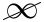
\includegraphics[width=0.4cm]{infbar}
}

\newcommand{\beginbackup}{
   \newcounter{framenumbervorappendix}
   \setcounter{framenumbervorappendix}{\value{framenumber}}
}
\newcommand{\backupend}{
   \addtocounter{framenumbervorappendix}{-\value{framenumber}}
   \addtocounter{framenumber}{\value{framenumbervorappendix}} 
}

\usefonttheme[onlymath]{serif}


\institute{INSA Rouen Normandie - Laboratoire LITIS}

% =================================================================================
\begin{document}
\maketitle

% =================================================================================

\begin{frame}{Outline}
  \tableofcontents
\end{frame}

\section{Introduction to Representation Learning}
\label{sec:intro}

\begin{frame}
  \frametitle{Limitations of others methods}
  \begin{block}{Analysis of classic ML}
    \begin{enumerate}
    \item Choose a dataset and a task
    \item Compute features from the data
    \item Learn the model on features
    \item Predict
    \end{enumerate}
  \end{block}

  \begin{block}{Problems}
    \begin{center}
      How can we be sure that our features are optimal ?
    \end{center}
    \begin{itemize}
    \item They define the latent space
    \item Model ability to learn is limited by these representations
    \end{itemize}
  \end{block}
  
\end{frame}

\begin{frame}
  \frametitle{Neural Networks and Deep Learning}
  \begin{block}{Motivation}
    \begin{itemize}
    \item End to end learning
    \item Let's the model to find the optimal representation according to a task
    \end{itemize}
  \end{block}
\begin{center}


  \only<1>{
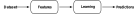
\includegraphics[width=.75\textwidth]{trad_ml}
}
\only<2>{
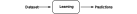
\includegraphics[width=.75\textwidth]{rl_ml}
}
\end{center}
\end{frame}


\section{Historical of Neural Networks}
\label{sec:histoire}

\begin{frame}[plain]
  \begin{center}
    {\Huge History of NN}
  \end{center}
  
\end{frame}

\begin{frame}
  \frametitle{How to simulate the human intelligence ?}
  \begin{block}{The human brain}
    \begin{itemize}
    \item Able to learn and adapt
    \item Simple neurons connected together
    \item Good connections are boosted
    \end{itemize}
  \end{block}
\end{frame}

\begin{frame}
  \frametitle{Brain Neuron}
  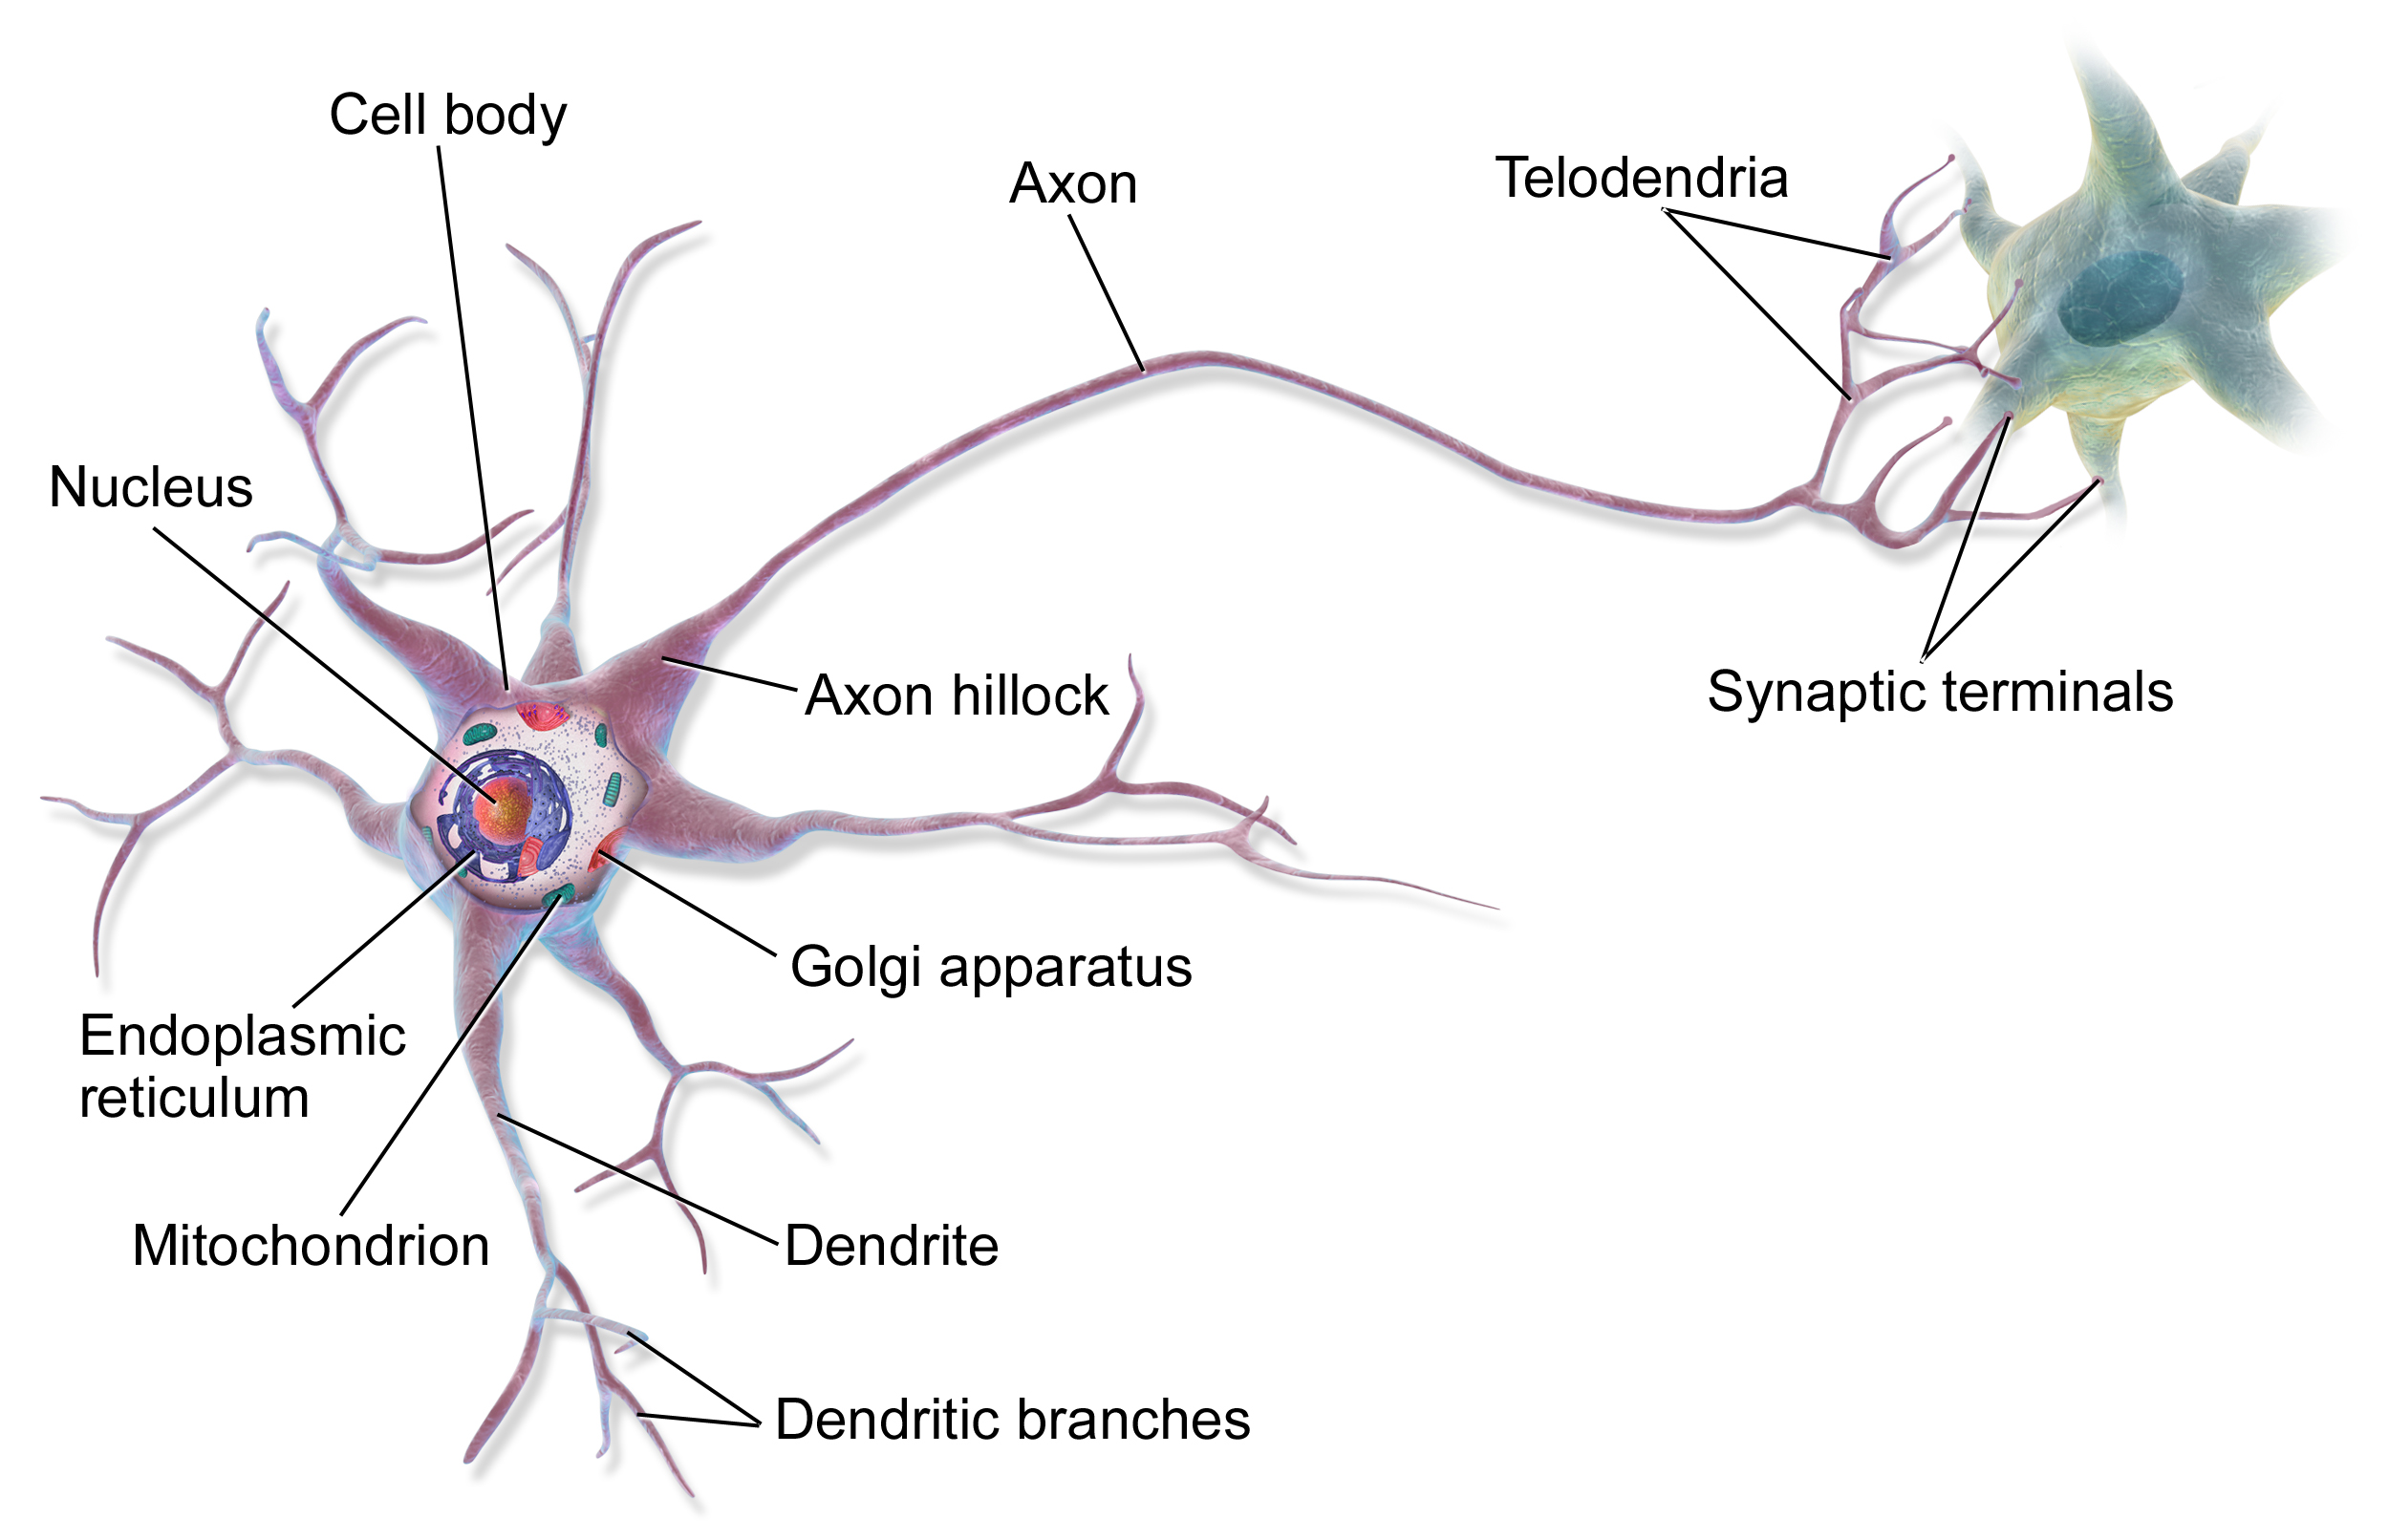
\includegraphics[width=\textwidth]{neurone_brain}
\end{frame}

\begin{frame}
  \frametitle{McCulloch Pitts (MCP) Neuron in 1943}
  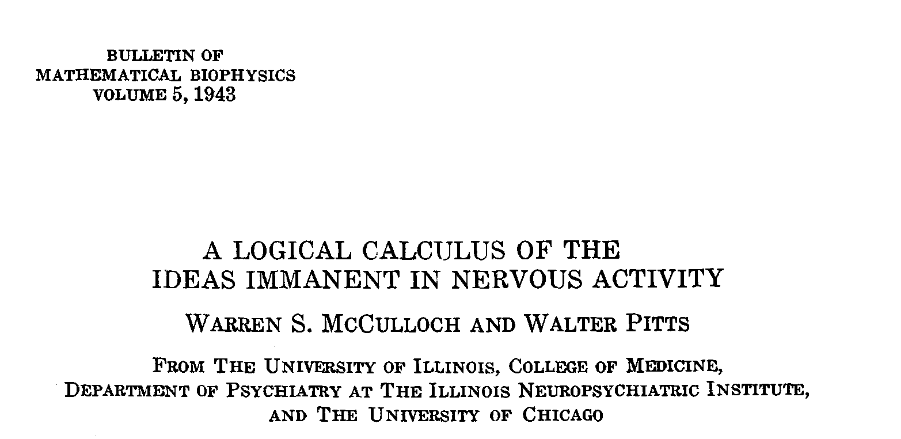
\includegraphics[width=\textwidth]{mcculloghpitts.png}
  \begin{itemize}
  \item A first simple approach
  \end{itemize}
\end{frame}

\begin{frame}
  \frametitle{The perceptron learning rule}
  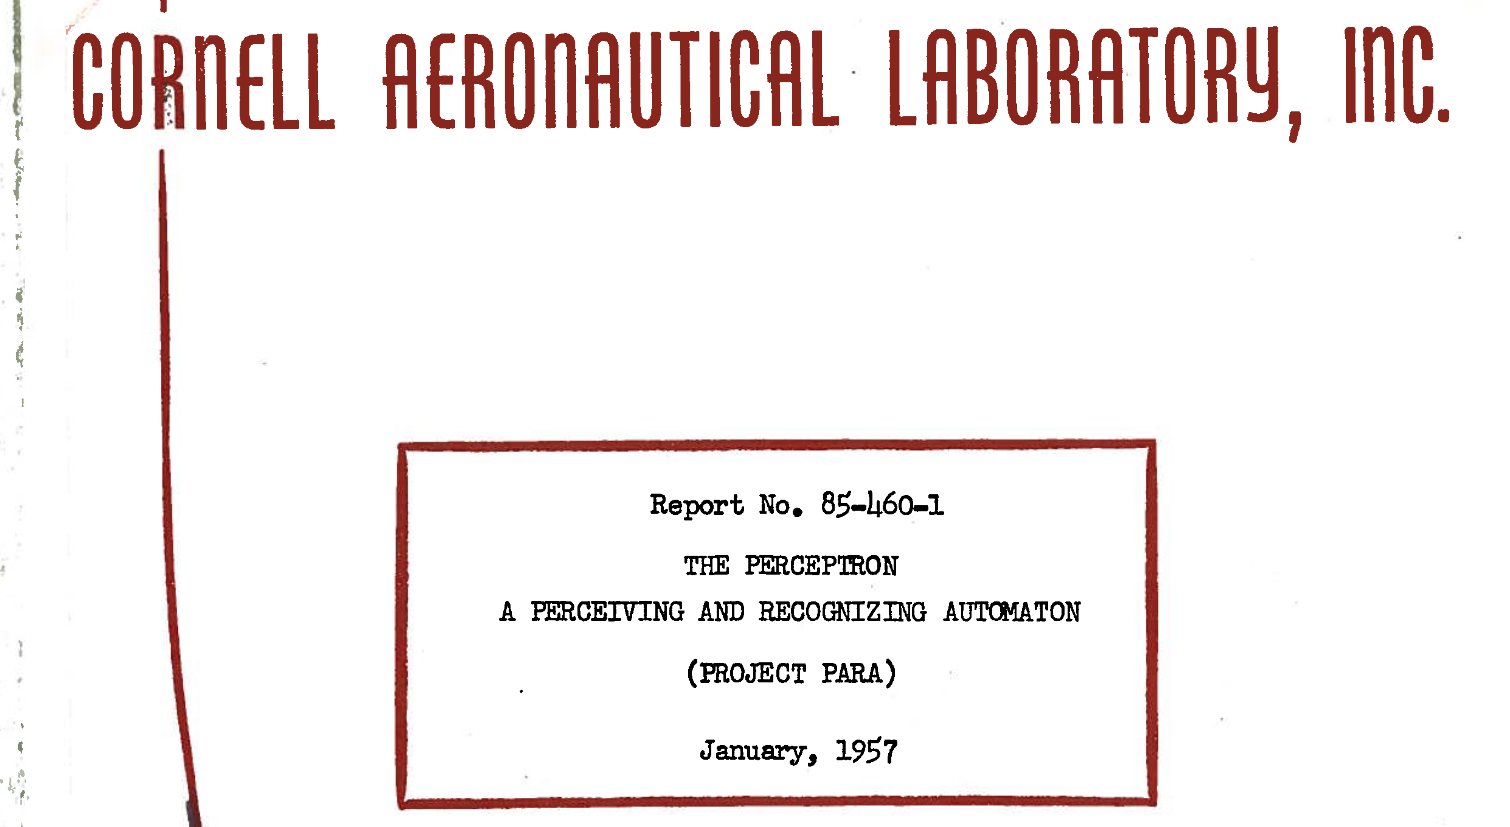
\includegraphics[width=.8\textwidth]{rosenblatt}
  \begin{itemize}
  \item The learning rule
  \item Basics of NN
  \end{itemize}
\end{frame}

\begin{frame}
  \frametitle{And then}
  \begin{columns}
    \begin{column}{.4\textwidth}
        \begin{itemize}
  \item Adaline 
  \item Multilayer Perceptron
  \item LeNet
  \item AlexNet
  \item \dots
  \end{itemize}
    \end{column}
    \begin{column}{.6\textwidth}
        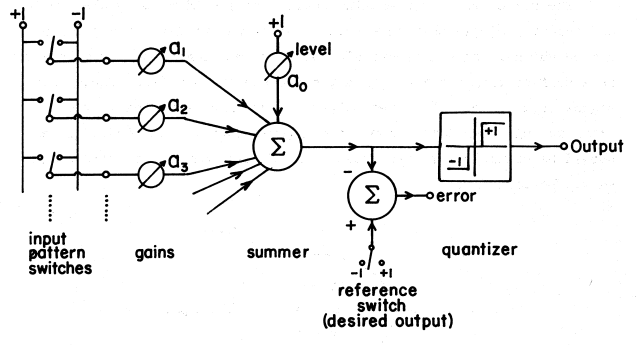
\includegraphics[width=\textwidth]{adaline}
    \end{column}
  \end{columns}
  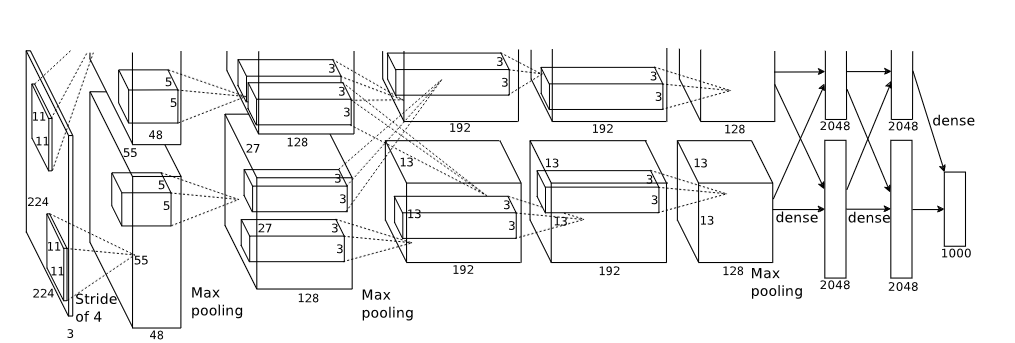
\includegraphics[width=\textwidth]{alexnet}
\end{frame}

\section{The Perceptron Model}
\label{sec:perceptron}
\begin{frame}[allowframebreaks]
  \frametitle{The Perceptron}
  \begin{block}{Artifical neurons}
    \begin{itemize}
    \item inputs $x$ : vector components
    \item weights $w$: how inputs are used
    \item output $z = w^\top x +b $ : net input
    \item Neuron fires if $z > 0$  i.e. $$\sigma(z) = \begin{cases}
       1 \text{ if } z > 0 \\
       0 \text{ otherwise }
     \end{cases}$$
    \end{itemize}
  \end{block}
  % Rajouter image
  \begin{block}{Perceptron Learning Rule}
    \begin{enumerate}
      \item Initialize weights to small random values
      \item For each training sample $\x_i$:
      \begin{enumerate}
        \item Compute the output value $\hat{y}$
        \item Update the weights
        \item Repeat until convergence
      \end{enumerate}
    \end{enumerate}
  \end{block}
  \begin{block}{How to update}
    \begin{itemize}
      \item Update the weights according to the error
      \item $ w_j = w_j + \Delta w_j$
      \item $\Delta w_j = \eta (y_i - \hat{y}_i) x_i(j)$
      \item $\eta$ is the learning rate
      \item $b = b + \Delta b, \Delta b = \eta (y_i - \hat{y}_i)$
    \end{itemize}
  \end{block}
  \begin{center}
    Let's try it !
  \end{center}

\begin{center}
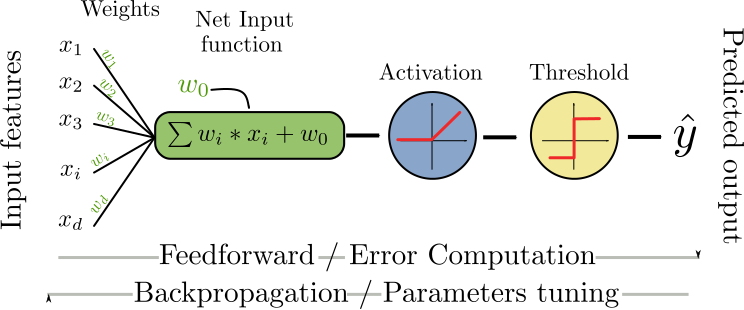
\includegraphics[width=\textwidth]{perceptron}
\end{center}
  
%% figure 2.4 p.25 Raschka

%% % exemple à la main de la descente de gradient

\end{frame}

\begin{frame}
  \frametitle{Adding some complexity}
  % Non linéarité
  \begin{block}{Linearity}
    The model is linear by design
    \begin{itemize}
    \item Add some linearities !
    \item $z = g(w^\top x + b)$
    \item $g$ is a differentiable function (ReLU, tanh, sigmoid, \dots)
    \end{itemize}
  \end{block}
  \begin{block}{Layers}
    Add more layers to complexify the interactions between the components of $x$
    \begin{itemize}
    \item Lead to Multi Layer Perceptron
    \item And \textbf{Deep} Learning
    \end{itemize}
  \end{block}
\end{frame} 

\section{The Multi Layer Perceptron}
\label{sec:mlp}

\begin{frame}{Multi Layer Perceptron}
  \begin{block}{Principle}
    Learn the best representation of data
    \vfill
    
\begin{figure}
  \centering
      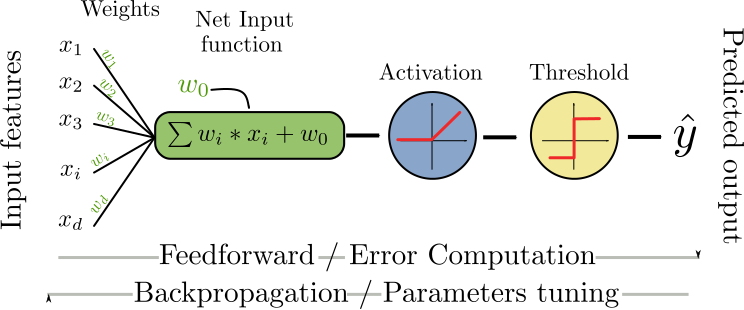
\includegraphics[width=\textwidth]{myperceptron}
\end{figure}
   
    \vfill
      \begin{itemize}
      \item Weights $\w$ are optimized by gradient descent
      \item Sequence of layers
      \end{itemize}
    \end{block}
\end{frame}

\begin{frame}[fragile]
  \frametitle{MLP Hyperparameters}

  \begin{block}{Hidden layers}
    Define the architecture of your MLP
    \begin{itemize}
    \item Number of layers : a high number tends to deep networks
    \item Number of neurons per layer : a high number tends to wide networks
    \end{itemize}
    The model will be more complex if more neurons are used
  \end{block}

  \begin{block}{Activation function}
    Determine how the non linearity is brought to the model
    \begin{itemize}
    \item identity : linear model
    \item tanh, relu, logistic : non linears. ReLU is a very popular choice
    \end{itemize}
  \end{block}

\end{frame}

\begin{frame}[fragile]
  \frametitle{MLP : the code !}
  
  \begin{minted}
[
frame=lines,
framesep=2mm,
baselinestretch=1.2,
fontsize=\footnotesize,
linenos
]
{python}
from sklearn.neural_network import MLPClassifier
activation = 'relu' # default
layers = [32,64,128,64,32] #5 layers avec différentes tailles
clf = MLPClassifier(hidden_layer_sizes=layers,max_iter=500)
clf.fit(X,y)
ypred = clf.predict(X)
\end{minted}

\begin{itemize}
\item User guide for tips and help :
  \href{https://scikit-learn.org/stable/modules/neural_networks_supervised.html#mlp-tips}{link}
  \item $\Rightarrow$ Notebook
%\item Exists for regression problems
  \item the
  \href{https://scikit-learn.org/stable/modules/generated/sklearn.neural_network.MLPClassifier.html}{documentation}
%% \item la
%%   \href{https://scikit-learn.org/stable/modules/svm.html#regression}{doc
%%     regressor}
\end{itemize}

\end{frame}
%% \begin{frame}
%%   \frametitle{The Multi Layer Perceptron}
%%   \begin{block}{Principle}
%%     \begin{itemize}
%%     \item Stack non linears layers
%%     \item A layer :
%%       \begin{itemize}
%%       \item An input size $m$
%%       \item A output size $d$
%%       \item An activation function (non linearity)
%%       \end{itemize}
%%     \end{itemize}
%%   \end{block}
%%   \begin{center}
%%   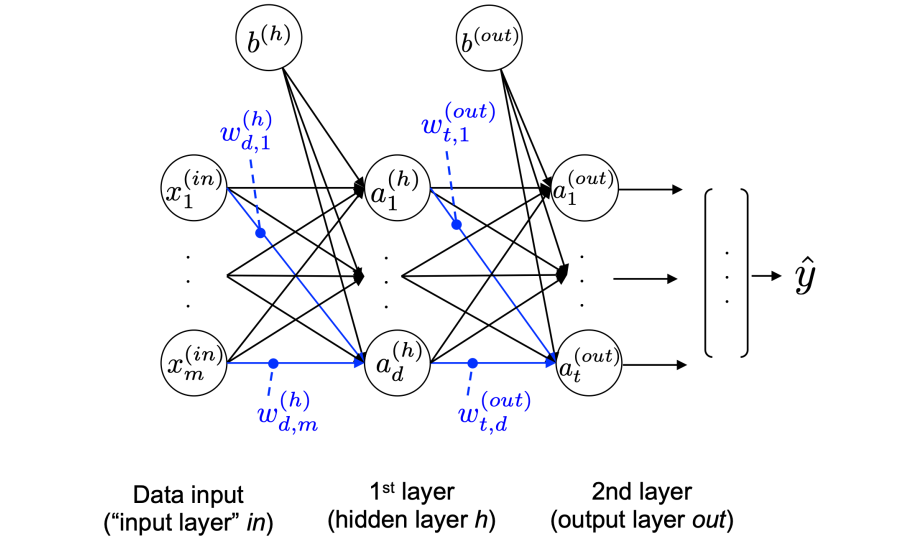
\includegraphics[width=.8\textwidth]{mlp}
%%   \end{center}
%% \end{frame}



%% \begin{frame}
%%   \frametitle{Backpropagation}
%%   \begin{block}{}
    
%%   \end{block}
%% \end{frame}

\begin{frame}
  \frametitle{Tensorflow playground}
  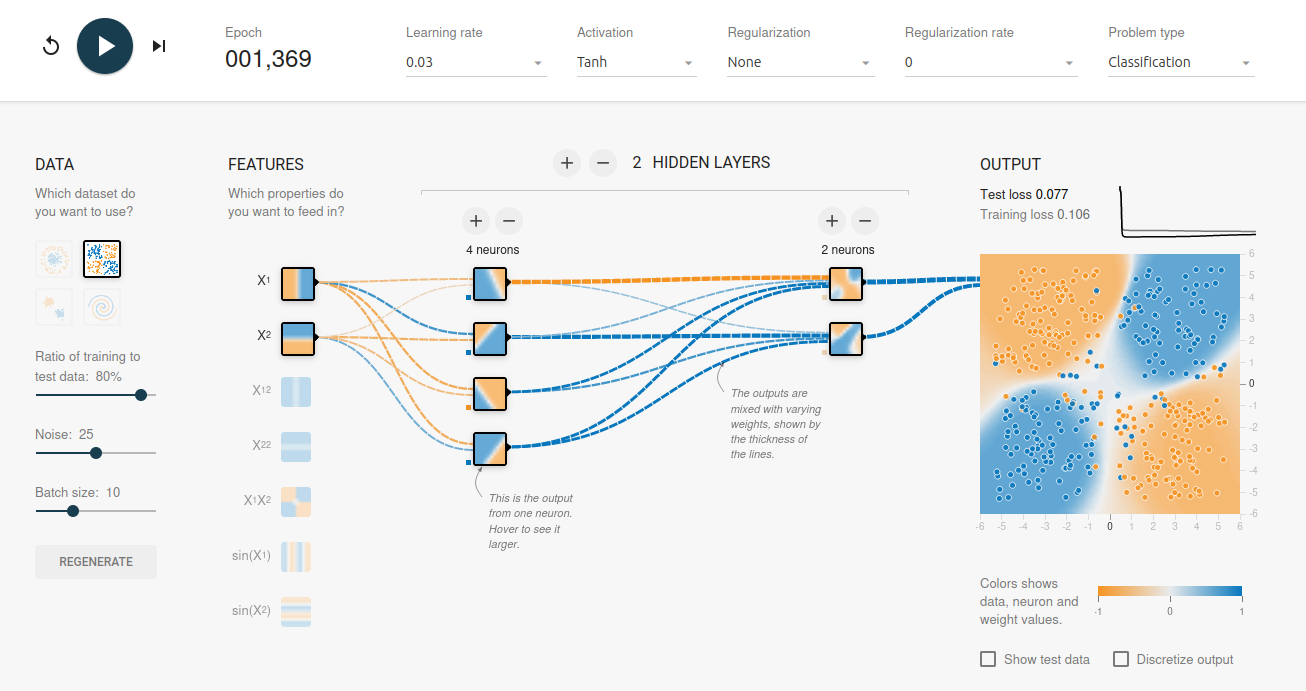
\includegraphics[width=\textwidth]{tensorflow}
  \url{https://playground.tensorflow.org/}
\end{frame}

\begin{frame}[fragile]
  \frametitle{Exemple with MNIST}
  $\rightarrow$ Notebook

  \begin{minted}
    [
      frame=lines,
      framesep=2mm,
      baselinestretch=1.2,
      fontsize=\footnotesize,
      linenos
    ]
    {python}
    
    import matplotlib.pyplot as plt
    from sklearn.datasets import load_digits
    from sklearn.neural_network import MLPClassifier
    from sklearn.model_selection import train_test_split

    X,y = load_digits(return_X_y = True)
    plt.imshow(X[124,:].reshape(8,8),cmap="gray")

    mlp = MLPClassifier(hidden_layer_sizes=(64,32,16),
        activation='relu',verbose=True)
    mlp.fit(X_train,y_train)
    X_train, X_test, y_train, y_test = train_test_split(X,y)
    from sklearn.metrics import accuracy_score
    print(accuracy_score(y_test,mlp.predict(X_test)))
    0.97777777... 
  \end{minted}
  
\end{frame}

\section{CNN, RNN etc}
\label{sec:cnnandco}

\begin{frame}
  \frametitle{Extension of MLP}
  \framesubtitle{How to learn on non tabular data ?}
  \begin{block}{Constraints}
    \begin{itemize}
    \item Data must be of fixed size dimensions
    \item Continuous
    \item All parts must be differentiable 
    \end{itemize}
  \end{block}

  \begin{block}{Nature of the data}
    \begin{itemize}
    \item How to take into account data topology ?
    \item Is MLP sufficient ? 
    \end{itemize}
  \end{block}
  
  
\end{frame}

\begin{frame}
  \frametitle{RNN : Adaptation to sequences}
  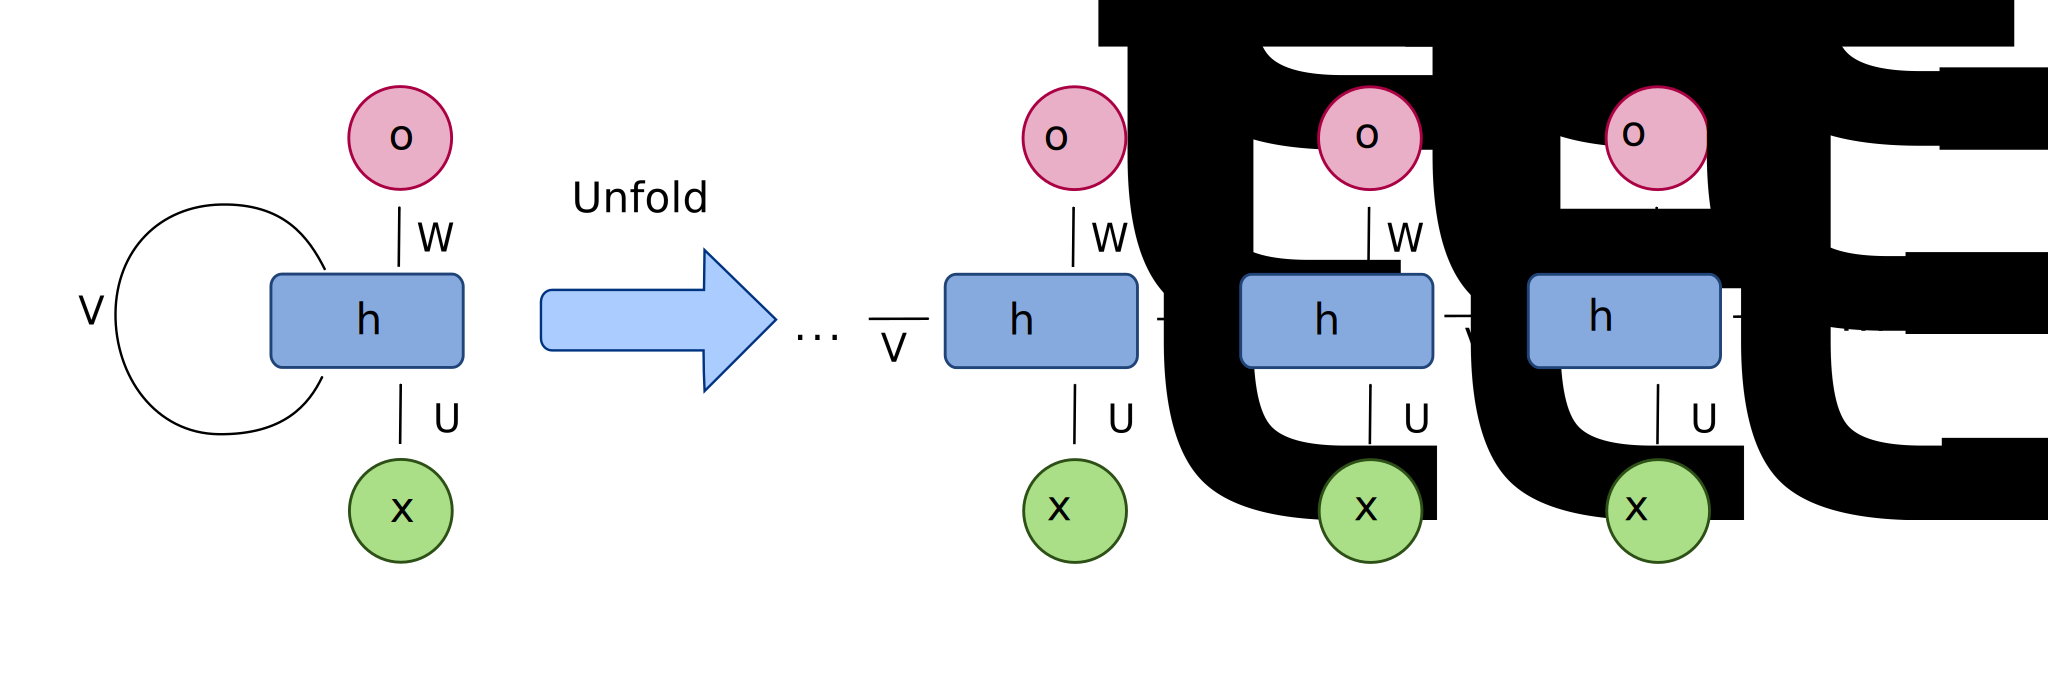
\includegraphics[width=\textwidth]{rnn}
                  {\footnotesize [wikipedia] }
                  
                  $\Rightarrow$ LSTM, GRU, \dots
\end{frame}

\begin{frame}
  \frametitle{CNN : Adaptation to images}
  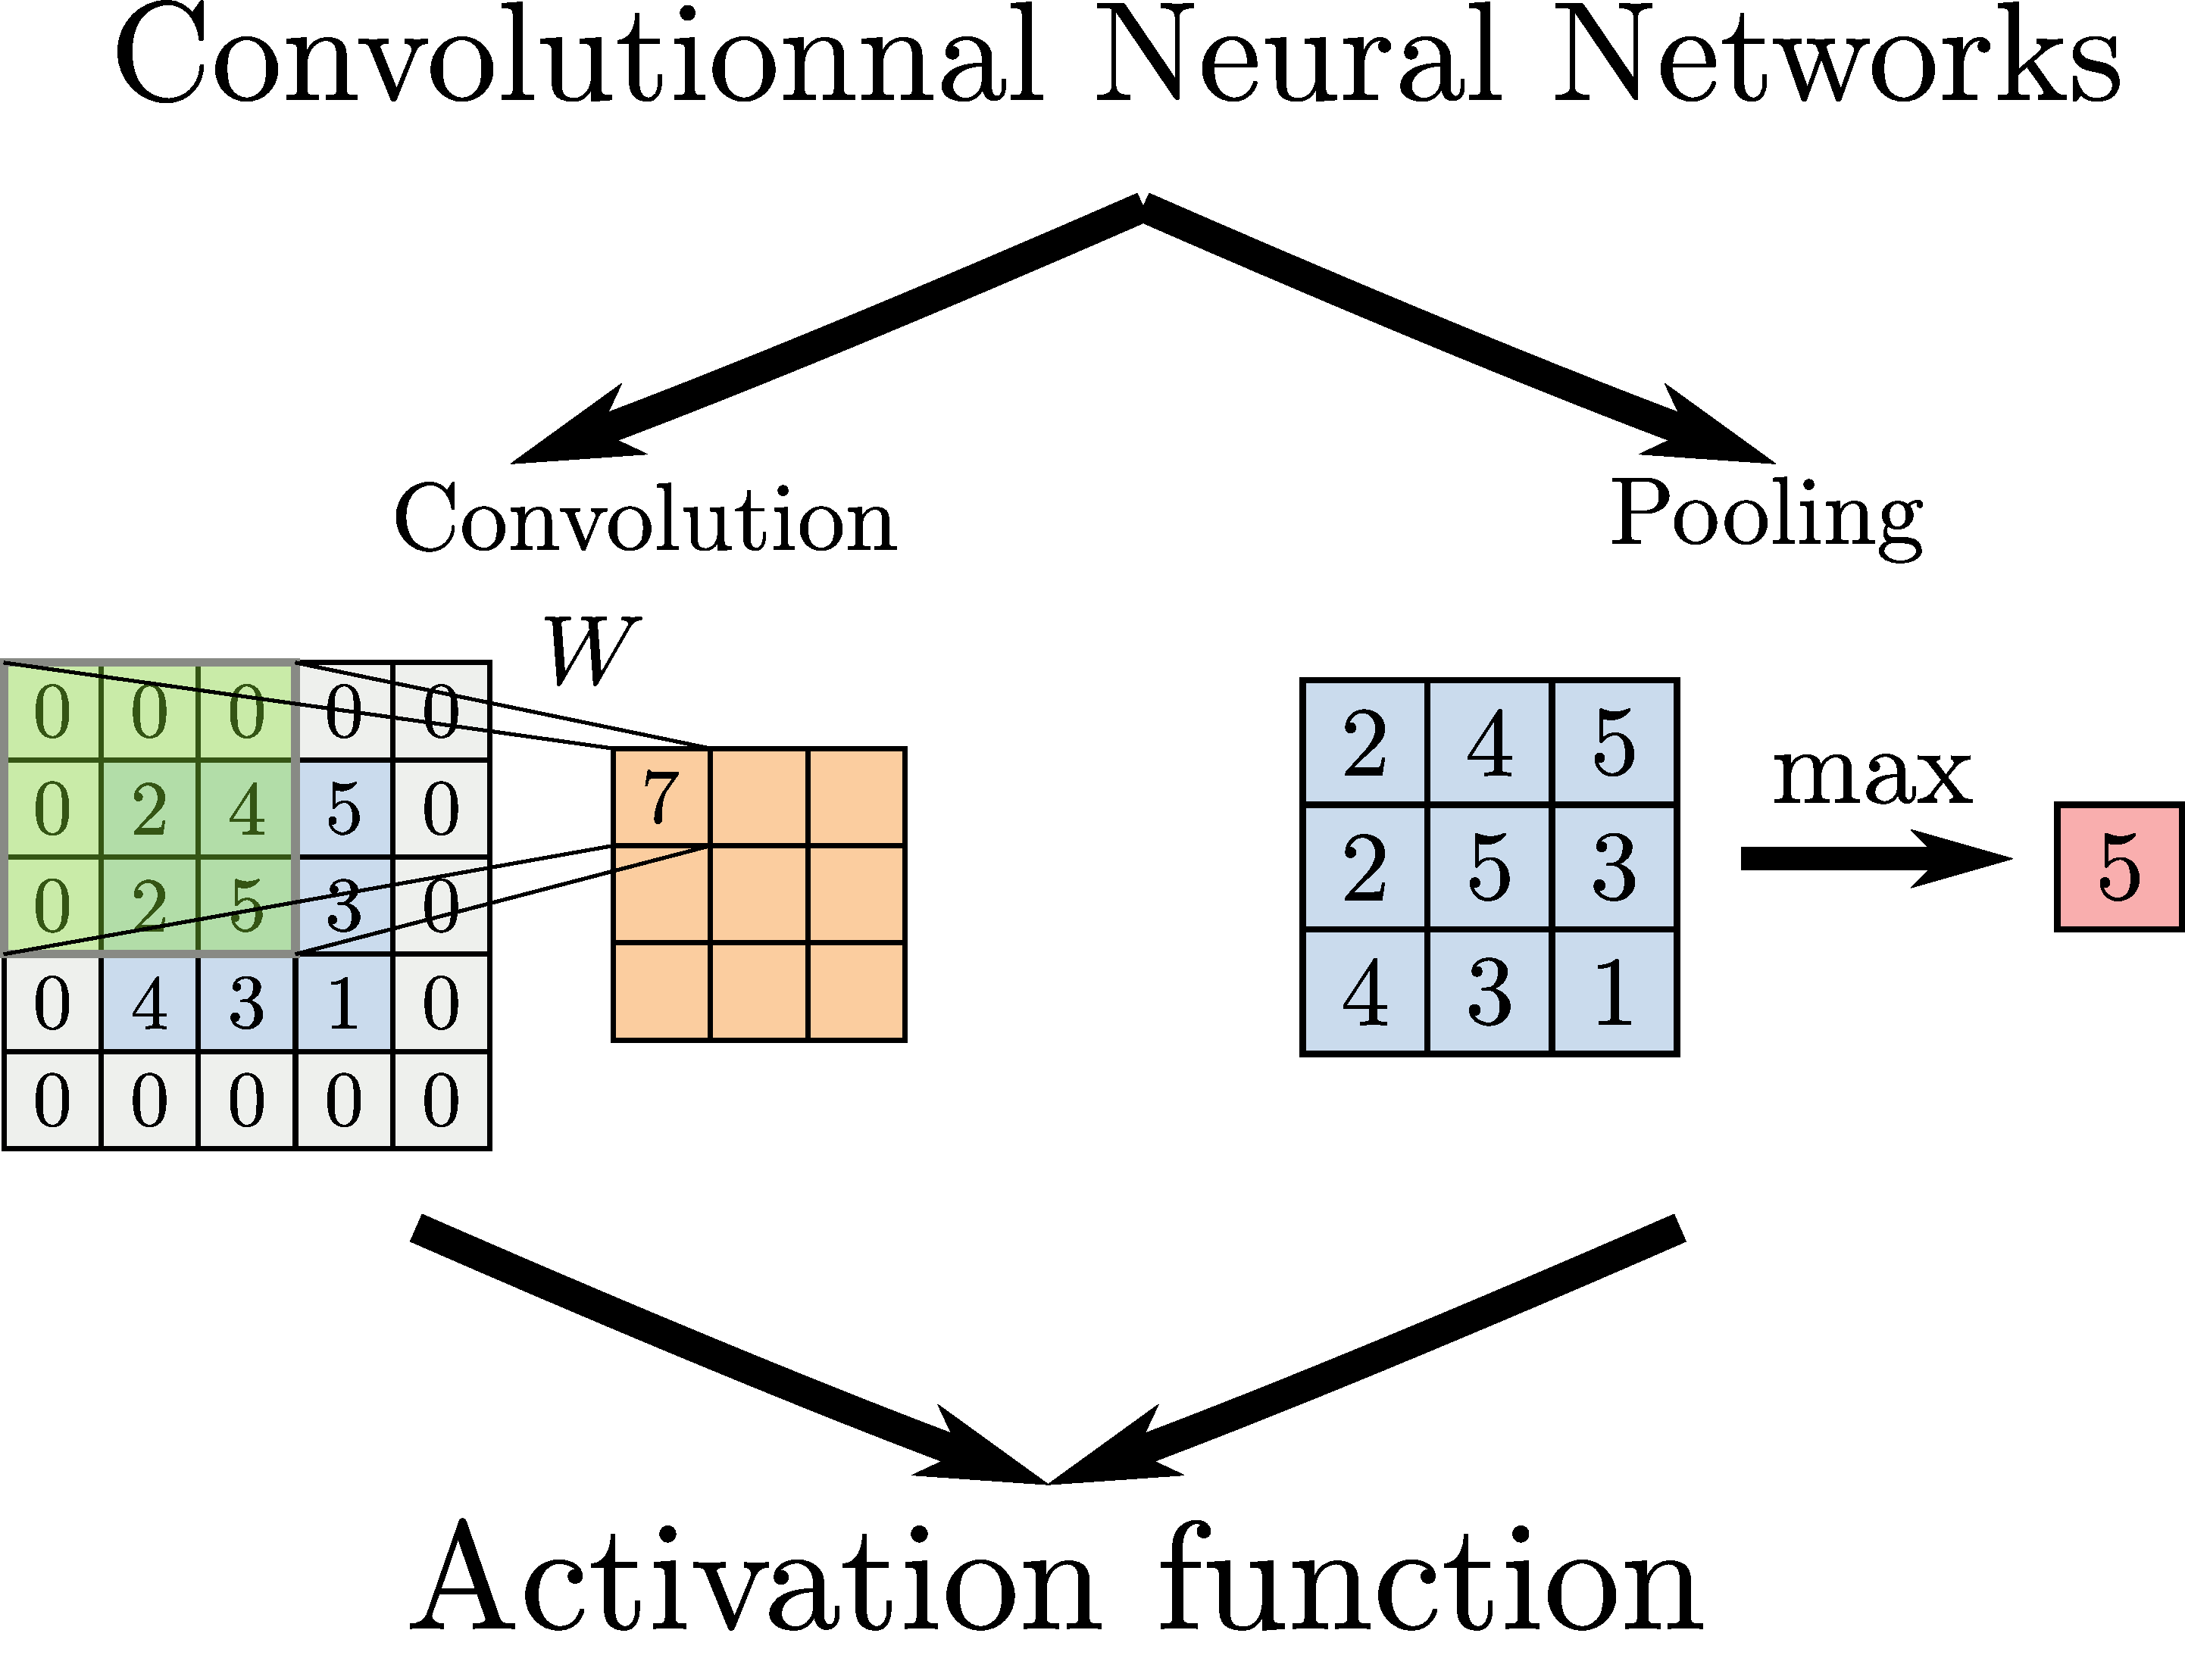
\includegraphics[width=\textwidth]{cnn}
\end{frame}


\begin{frame}
  \frametitle{And other things \dots}
  \begin{block}{Transformers}
    \begin{itemize}
    \item SOTA for NLP and Images
    \item GPT is for Generative Pretrained Transformer
    \item Embed the context to derive a better decision
    \end{itemize}
  \end{block}
  \begin{block}{Generative models}
    \begin{itemize}
    \item GAN
    \item Diffusion models
    \item dots
    \end{itemize}
  \end{block}
\end{frame}
\begin{frame}
  \frametitle{Conclusion}
  \begin{itemize}
  \item Neural Networks is a powerful ML method
  \item Paradigm shift : representation is learnt
  \item Strong results since 10 years
  \end{itemize}
  \begin{block}{What's next ?}
    \begin{center}
    {\Large How to adapt NN and CNN to molecules ? }
    \end{center}
  \end{block}

\end{frame}

% =================================================================================
\nocite{*}
\begin{frame}
  \frametitle{References}
    \begin{block}{References}
      \bibliographystyle{plainnat}
      \bibliography{biblio_nn}
  \end{block}
\end{frame}



\end{document}
